\section{Anexos}

\subsection{Anexo A: Evidencia de Capacitaciones al Personal del CRM}

El presente anexo reúne el registro fotográfico y documental de las sesiones de capacitación impartidas al personal y la gerencia de Machu Picchu Exclusive Tours E.I.R.L. en el uso del sistema ERP Odoo 19. Las capacitaciones abarcaron los módulos de CRM Turístico, gestión de contactos, control de itinerarios (Proyectos/Kanban), ventas, cotizaciones y buenas prácticas de seguridad de la información.

\subsubsection{A.1 Registro fotográfico de capacitaciones presenciales}

\begin{indentedsubsection}
Las siguientes fotografías documentan las sesiones de capacitación presencial realizadas con la gerencia general y el equipo operativo en las instalaciones de la empresa. Estas sesiones se centraron en la adopción práctica del sistema Odoo para la gestión del CRM turístico, el control de reservas e itinerarios y el seguimiento de actividades.

\begin{figure}[H]
    \centering
    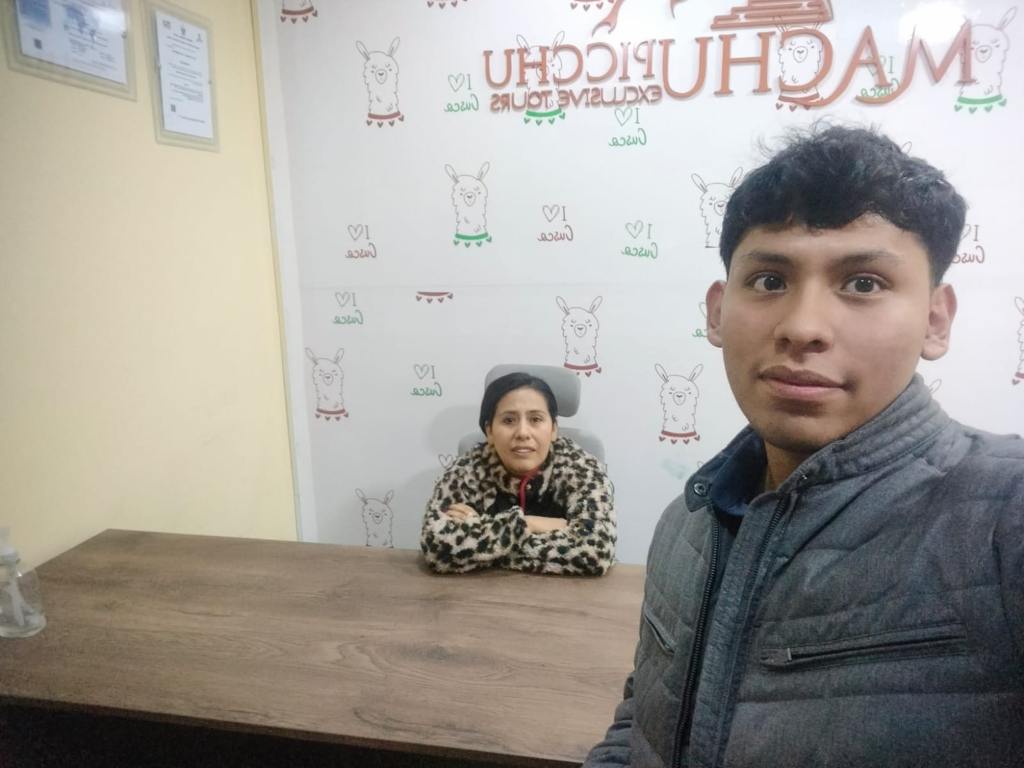
\includegraphics[width=0.85\textwidth]{../InformeImplementacionMachuPicchu/assets/capacitacion-presencial-1.png}
    \caption{Sesión práctica presencial: coordinación operativa y configuración inicial del sistema Odoo 19 con la gerencia de Machu Picchu Exclusive Tours.}
\end{figure}

\begin{figure}[H]
    \centering
    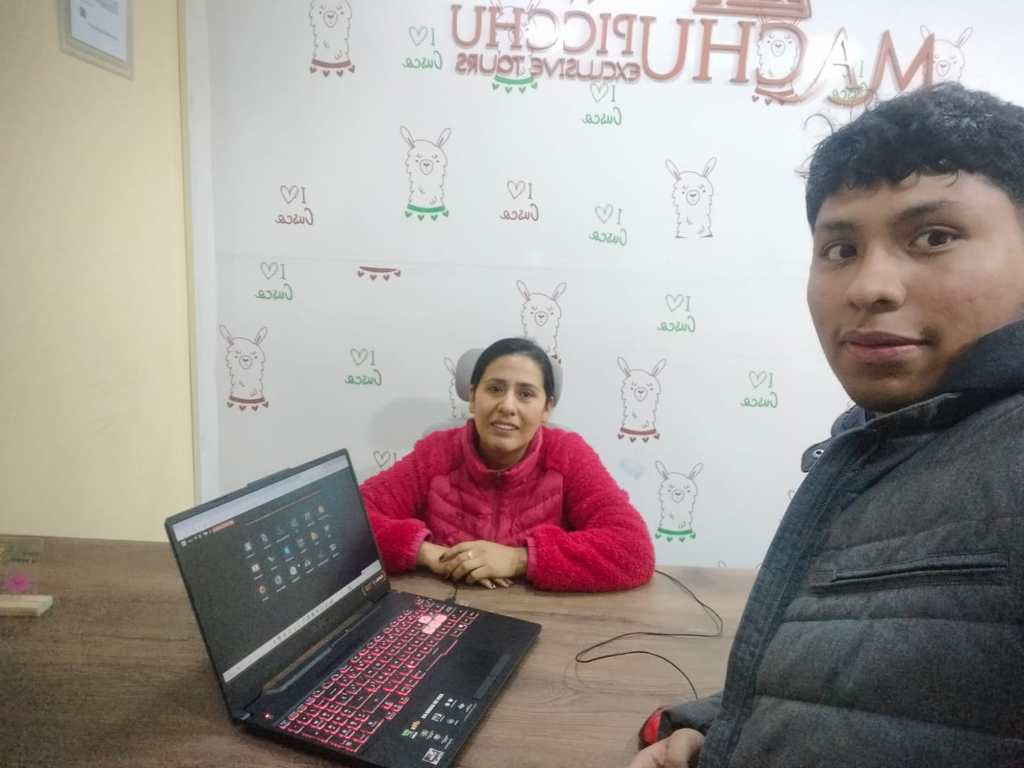
\includegraphics[width=0.85\textwidth]{../InformeImplementacionMachuPicchu/assets/capacitacion-presencial-2.png}
    \caption{Capacitación interactiva presencial: entrenamiento en la interfaz de Odoo para el control de reservas, gestión del pipeline CRM y administración de itinerarios turísticos.}
\end{figure}

\end{indentedsubsection}

\subsubsection{A.2 Registro de capacitación virtual y asistencia remota}

\begin{indentedsubsection}
Complementariamente a las sesiones presenciales, se realizaron sesiones de capacitación virtual y asistencia remota para reforzar el uso del sistema y guiar a los usuarios en la navegación por los módulos de CRM, Contactos, Ventas y Proyectos. Este formato permitió resolver dudas operativas en tiempo real sin necesidad de desplazamiento.

\begin{figure}[H]
    \centering
    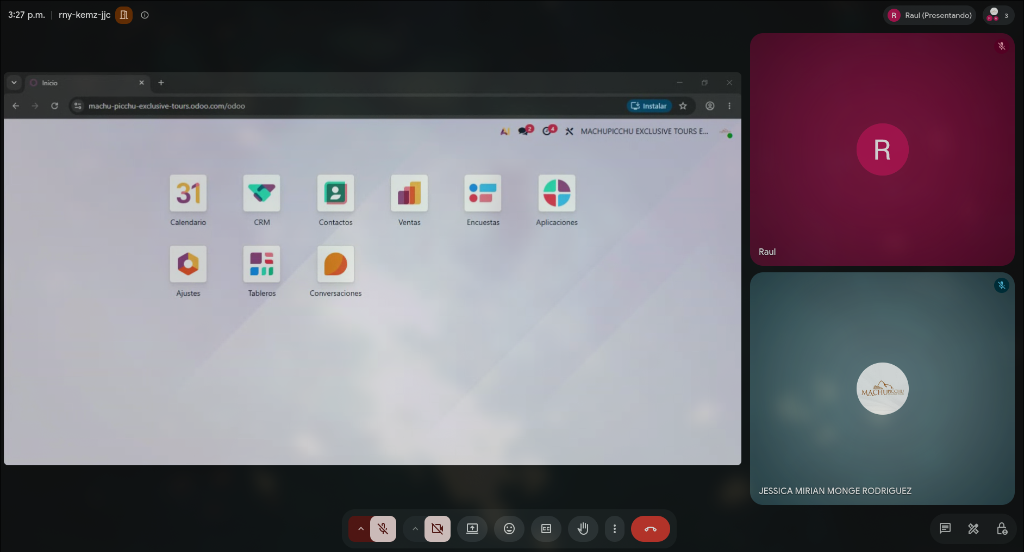
\includegraphics[width=0.85\textwidth]{../InformeImplementacionMachuPicchu/assets/capacitacion-virtual-1.png}
    \caption{Sesión de capacitación virtual remota: revisión del entorno Odoo de la empresa, navegación por módulos y resolución de dudas operativas de la gerencia general.}
\end{figure}

\begin{figure}[H]
    \centering
    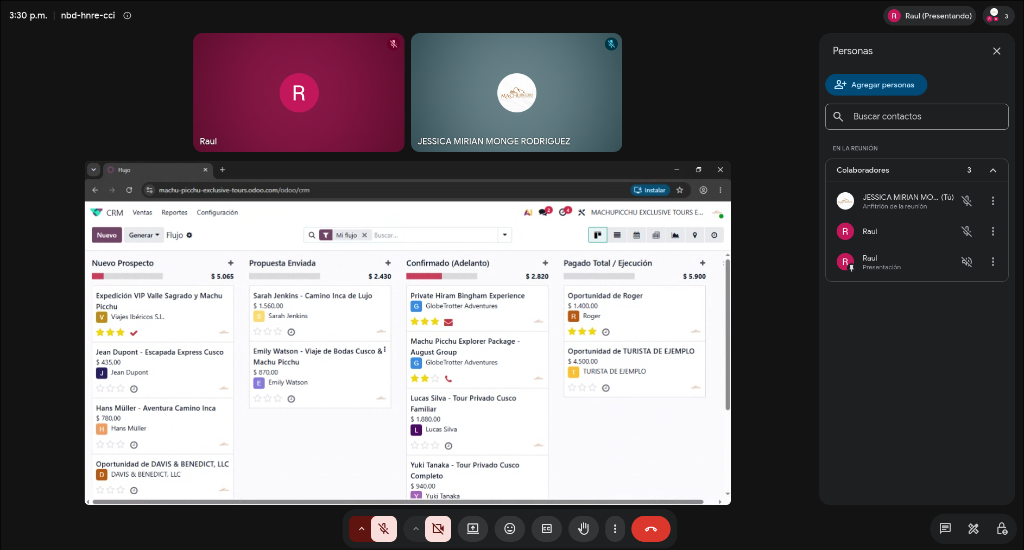
\includegraphics[width=0.85\textwidth]{../InformeImplementacionMachuPicchu/assets/capacitacion-virtual-2.png}
    \caption{Taller virtual práctico: capacitación en el control de flujos CRM, gestión del pipeline turístico y registro de adelantos de pago en el módulo de Ventas.}
\end{figure}

\end{indentedsubsection}

\subsubsection{A.3 Resumen de sesiones de capacitación ejecutadas}

\begin{indentedsubsection}
La siguiente tabla sintetiza las sesiones de capacitación efectivamente ejecutadas durante el proyecto, con indicación de los participantes, temas cubiertos y modalidad:

\renewcommand{\arraystretch}{1.35}
\begin{longtable}{|p{2.2cm}|p{3.0cm}|p{2.5cm}|p{5.0cm}|p{1.5cm}|}
\hline
\textbf{Modalidad} & \textbf{Participante(s)} & \textbf{Rol} & \textbf{Temas cubiertos} & \textbf{Horas} \\ \hline
\endfirsthead
\hline
\textbf{Modalidad} & \textbf{Participante(s)} & \textbf{Rol} & \textbf{Temas cubiertos} & \textbf{Horas} \\ \hline
\endhead
Presencial & Jessica M. Monge Rodríguez & Gerente General (usuaria principal) & Acceso a Odoo Online, configuración base, buenas prácticas de seguridad de la información & 2 \\ \hline
Presencial & Jessica M. Monge Rodríguez & Gerente General & Gestión de clientes y contactos: registro de PAX, carga de documentos de identidad, historial comercial & 3 \\ \hline
Presencial & Jessica M. Monge Rodríguez & Gerente General & CRM y embudo comercial: creación de oportunidades, cambio de etapas, bitácora, transición a cotizaciones & 3 \\ \hline
Presencial & Jessica M. Monge Rodríguez & Gerente General & Ventas y cotizaciones: emisión desde CRM, confirmación de adelantos, configuración de tours & 4 \\ \hline
Virtual & Jessica M. Monge Rodríguez & Gerente General & Encuestas de satisfacción y cierre operativo: aplicación, lectura de resultados, buenas prácticas & 2 \\ \hline
Virtual & Jessica M. Monge Rodríguez & Gerente General & Repaso flujo completo CRM-Ventas-Proyectos y resolución de dudas operativas en tiempo real & 2 \\ \hline
\multicolumn{4}{|r|}{\textbf{Total de horas de capacitación ejecutadas:}} & \textbf{16 h} \\ \hline
\end{longtable}

\end{indentedsubsection}

\newpage
\subsection{Anexo B: Capturas de Pantalla del Sistema Odoo 19 en Producción}

El presente anexo presenta capturas de pantalla reales del sistema Odoo 19 operativo en la nube (SaaS) de Machu Picchu Exclusive Tours E.I.R.L. (\texttt{machu-picchu-exclusive-tours.odoo.com}), tomadas durante el período de evaluación del proyecto. Estas evidencias demuestran el uso activo de los módulos implementados.

\subsubsection{B.1 Pipeline CRM — Vista Kanban}

\begin{indentedsubsection}
La siguiente captura muestra el pipeline CRM activo con oportunidades reales de la empresa organizadas en las cuatro etapas del flujo turístico: \textbf{Nuevo Prospecto}, \textbf{Propuesta Enviada}, \textbf{Confirmado (Adelanto)} y \textbf{Pagado Total / Ejecución}. Se evidencia la gestión de clientes internacionales (Viajes Ibéricos S.L., GlobeTrotter Adventures, Sarah Jenkins, Jean Dupont, Hans Müller, Lucas Silva, Yuki Tanaka) con un total de ingresos proyectados de \textbf{\$16,215.00 USD}.

\begin{figure}[H]
    \centering
    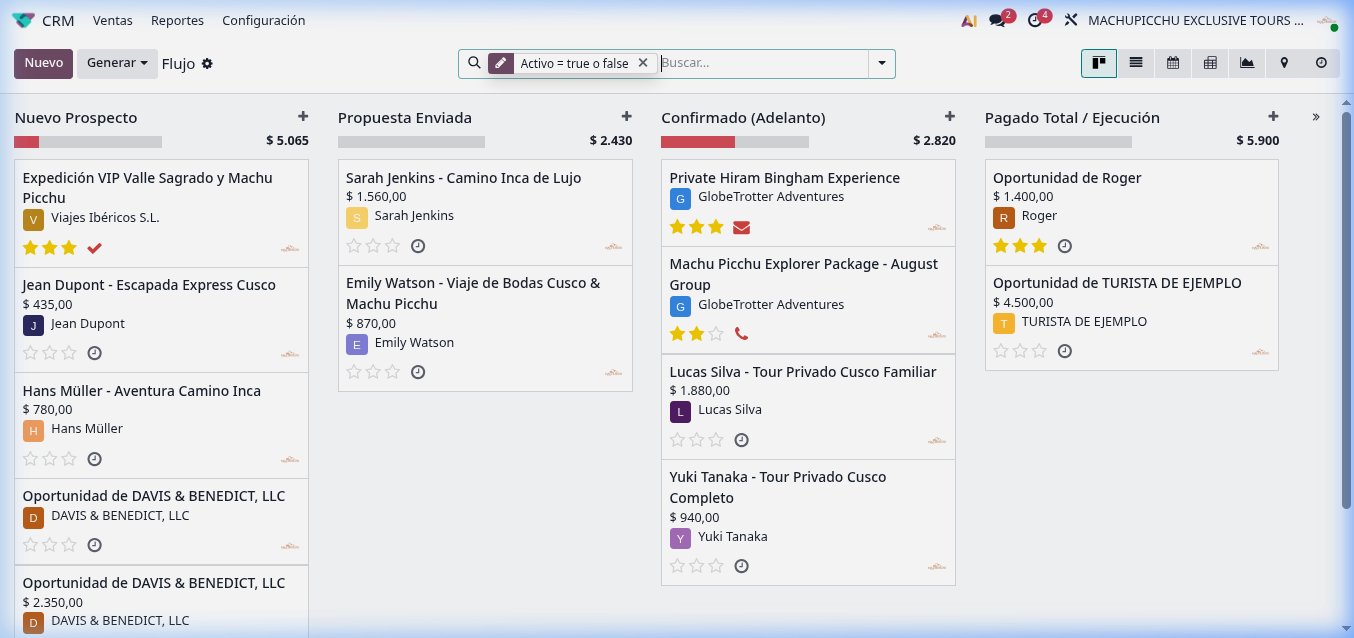
\includegraphics[width=\textwidth]{assets/odoo-crm-pipeline-real.png}
    \caption{Pipeline CRM Kanban activo en Odoo 19 --- Machu Picchu Exclusive Tours E.I.R.L. (captura real del sistema en producción, julio 2026). Se visualizan 14 oportunidades distribuidas en 4 etapas del flujo comercial.}
\end{figure}
\end{indentedsubsection}

\subsubsection{B.2 Pipeline CRM — Vista Lista de Oportunidades}

\begin{indentedsubsection}
La vista lista complementa el Kanban mostrando el detalle de las 14 oportunidades registradas, incluyendo el contacto asociado, correo electrónico, ingreso esperado y etapa actual. Se evidencia el uso sistemático del CRM para registrar y dar seguimiento a clientes de España, Francia, Alemania, Estados Unidos, Brasil y Japón.

\begin{figure}[H]
    \centering
    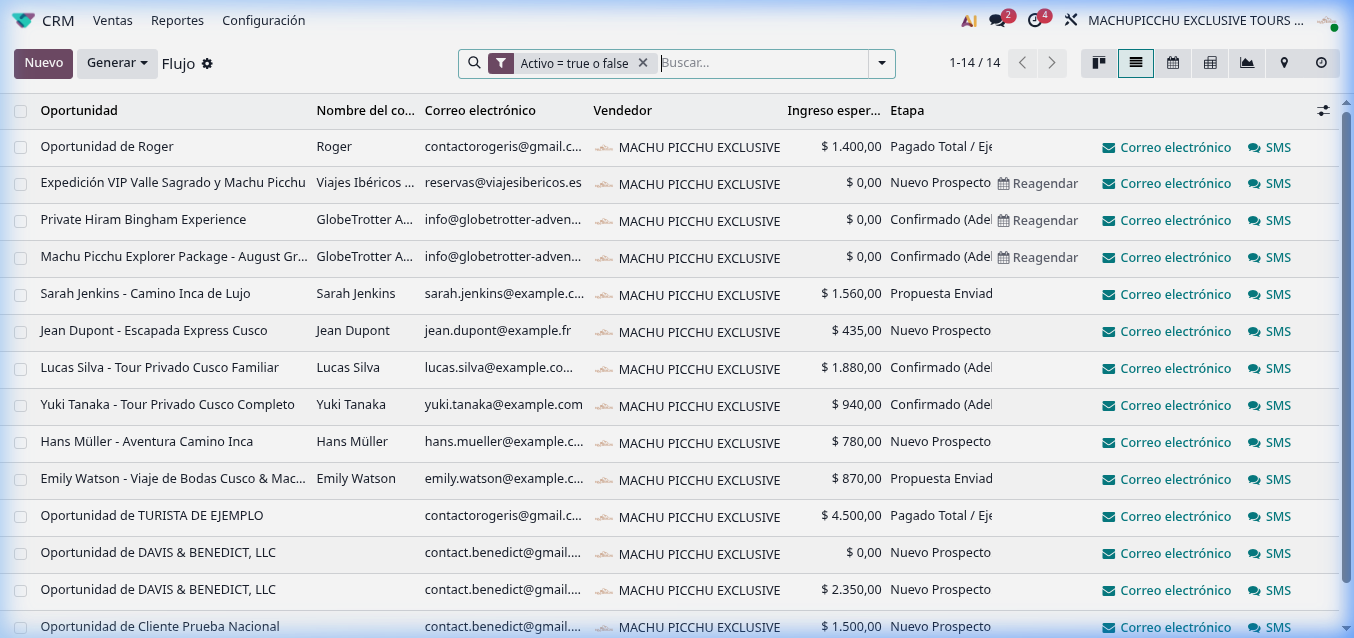
\includegraphics[width=\textwidth]{assets/odoo-crm-lista-real.png}
    \caption{Vista lista del CRM en Odoo 19 mostrando las 14 oportunidades activas con sus respectivos datos de contacto, correo, ingreso esperado y etapa de seguimiento (captura real del sistema, julio 2026).}
\end{figure}
\end{indentedsubsection}

\subsubsection{B.3 Ficha de Oportunidad con Trazabilidad de Actividades}

\begin{indentedsubsection}
La siguiente captura muestra una ficha de oportunidad real (``Expedición VIP Valle Sagrado y Machu Picchu'' --- Cliente: Viajes Ibéricos S.L.) con el historial de actividades en el chatter. Se evidencia la trazabilidad completa del flujo: desde la creación del lead, los cambios de etapa registrados automáticamente y las actividades planificadas por el sistema.

\begin{figure}[H]
    \centering
    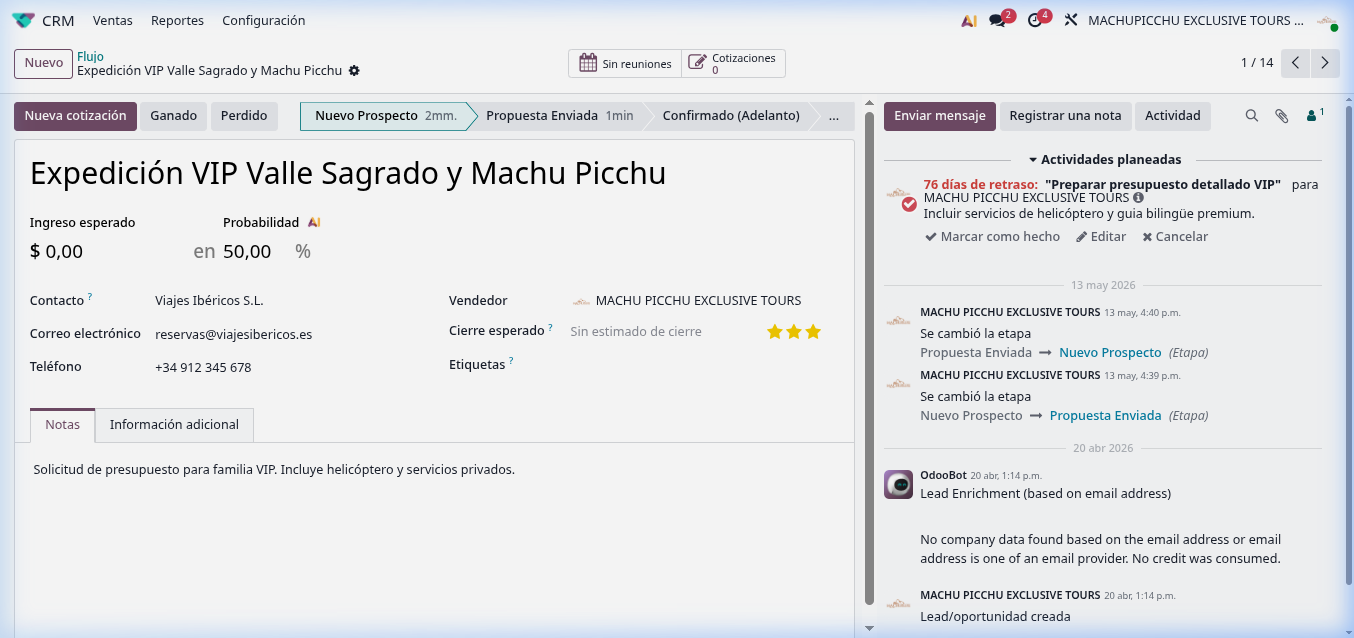
\includegraphics[width=\textwidth]{assets/odoo-crm-oportunidad-real.png}
    \caption{Ficha de oportunidad CRM ``Expedición VIP Valle Sagrado y Machu Picchu'' con trazabilidad completa de actividades en el chatter. Se evidencia el seguimiento de etapas y actividades pendientes (captura real del sistema, julio 2026).}
\end{figure}
\end{indentedsubsection}

\subsubsection{B.4 Módulo de Ventas — Cotizaciones y Órdenes de Venta}

\begin{indentedsubsection}
El módulo de Ventas muestra las 12 cotizaciones generadas, de las cuales 3 ya se convirtieron en \textbf{Órdenes de Venta} confirmadas (S00015: \$4,500.00, S00013: \$1,400.00, S00010: \$1,500.00). El total acumulado en el sistema asciende a \textbf{\$25,865.00 USD}, evidenciando el uso activo del control financiero.

\begin{figure}[H]
    \centering
    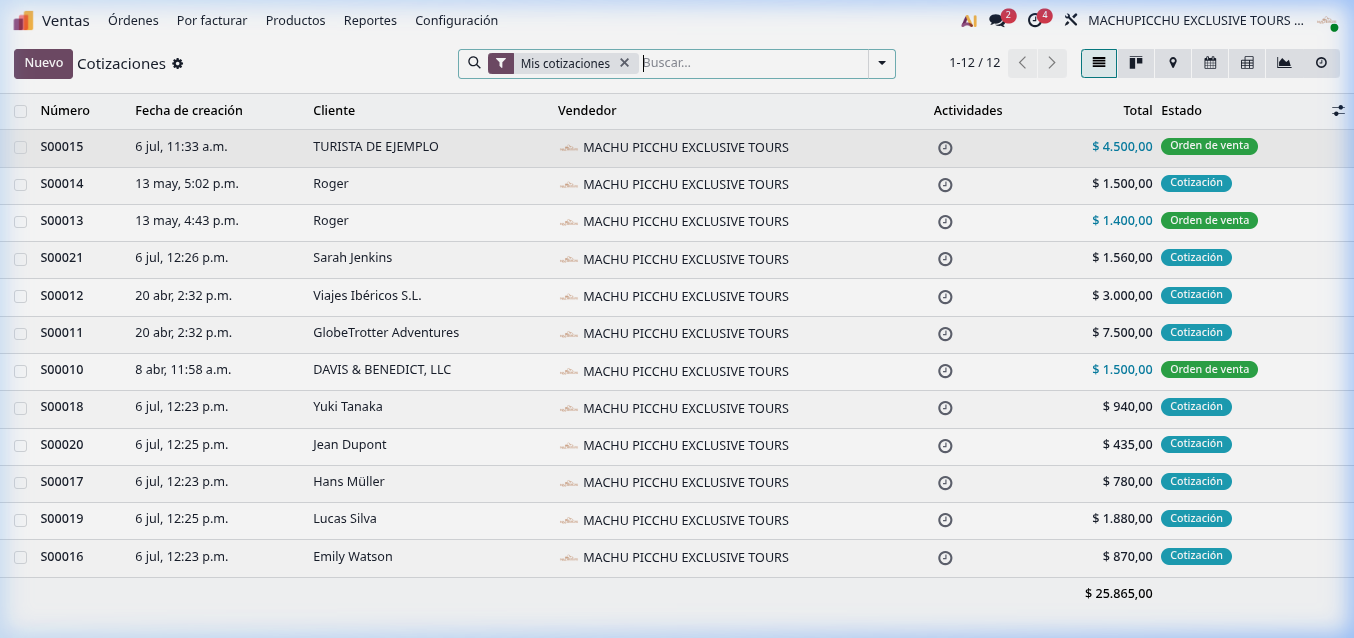
\includegraphics[width=\textwidth]{assets/odoo-ventas-real.png}
    \caption{Módulo de Ventas en Odoo 19 con 12 cotizaciones activas y 3 órdenes de venta confirmadas, por un total de \$25,865.00 USD. Se evidencia el control de adelantos y saldos por cliente (captura real del sistema, julio 2026).}
\end{figure}
\end{indentedsubsection}

\subsubsection{B.5 Módulo de Contactos — Base de Datos de Clientes (PAX)}

\begin{indentedsubsection}
El módulo de Contactos muestra la base de datos centralizada de 14 clientes internacionales registrados en el sistema, con sus datos de contacto, correo electrónico, teléfono y país de origen. Se evidencia la diversidad de mercados atendidos: Estados Unidos, España, Francia, Alemania, Brasil, Reino Unido, Japón y Perú.

\begin{figure}[H]
    \centering
    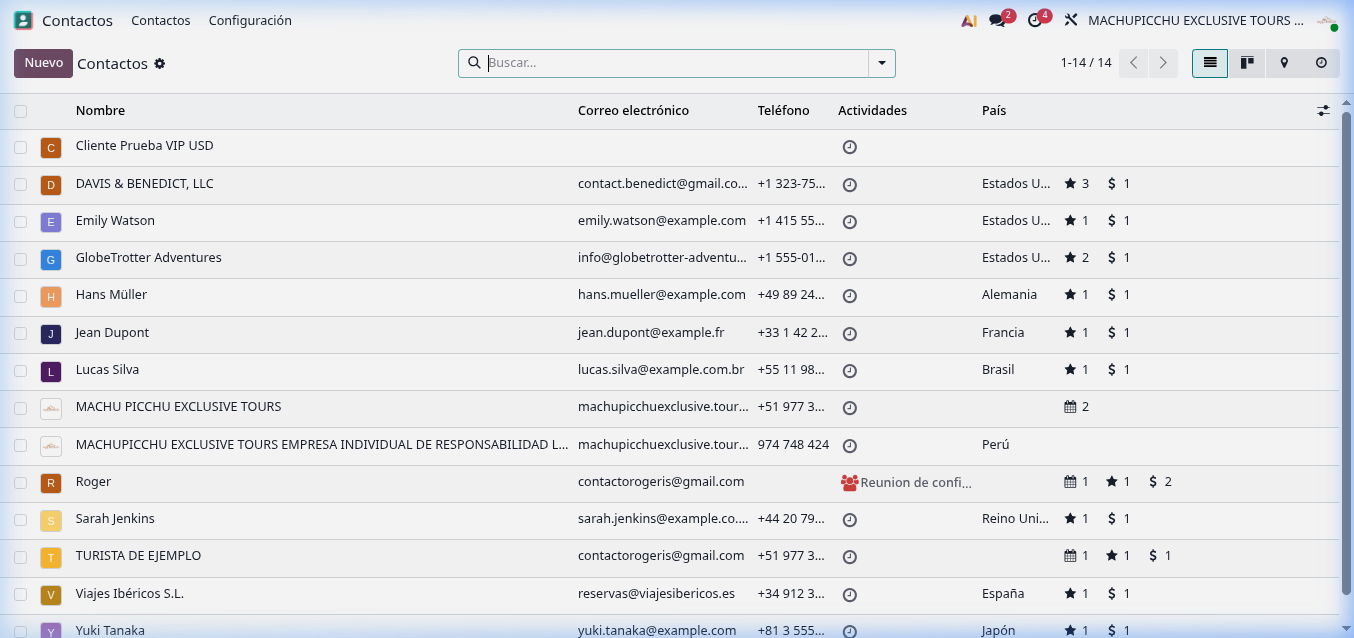
\includegraphics[width=\textwidth]{assets/odoo-contactos-real.png}
    \caption{Base de datos centralizada de contactos en Odoo 19 con 14 clientes internacionales registrados. Se elimina la dispersión previa de datos en WhatsApp y Excel (captura real del sistema, julio 2026).}
\end{figure}
\end{indentedsubsection}

\subsubsection{B.6 Módulo de Encuestas — Encuesta de Satisfacción Post-Tour}

\begin{indentedsubsection}
El módulo de Encuestas registra la ``Encuesta de Satisfacción --- Machu Picchu Exclusive Tours'' con 5 preguntas y \textbf{3 respuestas terminadas}, evidenciando el inicio de la estrategia de fidelización y medición de la satisfacción del cliente post-viaje.

\begin{figure}[H]
    \centering
    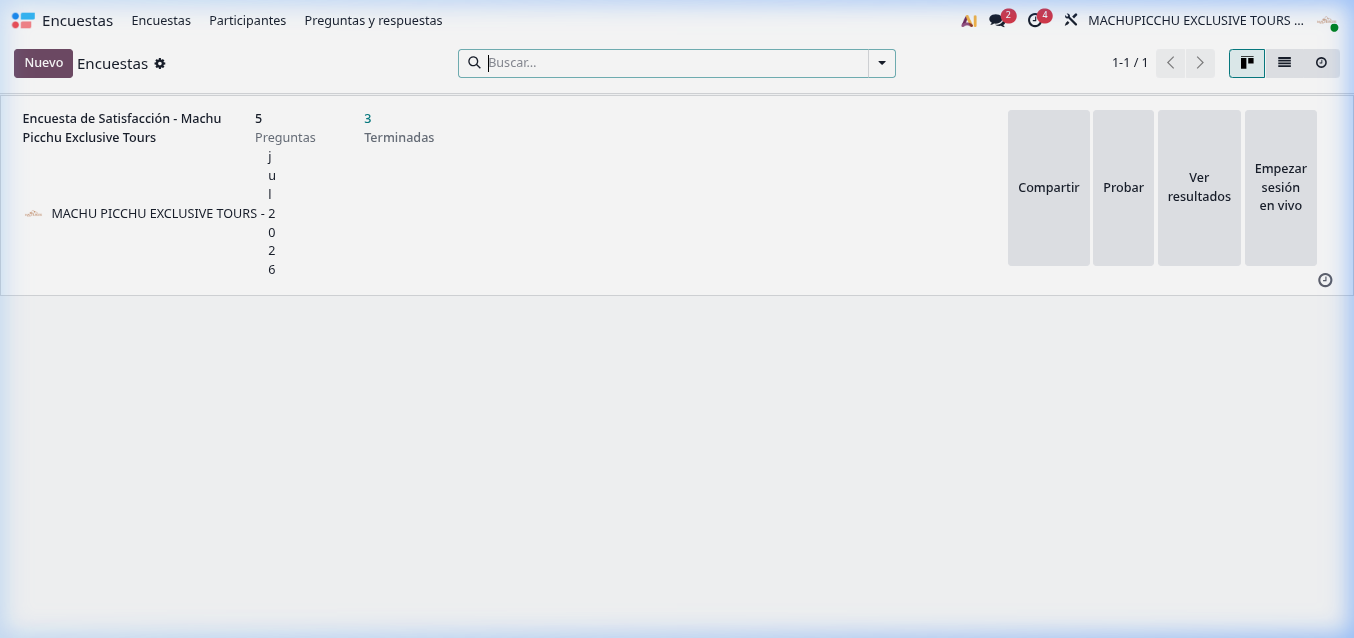
\includegraphics[width=0.9\textwidth]{assets/odoo-encuestas-real.png}
    \caption{Módulo de Encuestas en Odoo 19 con encuesta de satisfacción activa y 3 respuestas de clientes registradas, herramienta clave para medir la tasa de recomendación y fidelización (captura real del sistema, julio 2026).}
\end{figure}
\end{indentedsubsection}

\subsubsection{B.7 Análisis del Flujo CRM — Reporte de Pipeline por Etapas}

\begin{indentedsubsection}
El reporte ``Análisis del Flujo'' muestra la distribución de oportunidades por etapa del pipeline a lo largo del tiempo (2026). Se evidencia la concentración de 6 oportunidades en ``Nuevo Prospecto'', 2 en ``Propuesta Enviada'', 4 en ``Confirmado (Adelanto)'' y 2 en ``Pagado Total / Ejecución'', con una tasa de conversión acumulada del 28.6\% (4 de 14 oportunidades en etapas avanzadas o cerradas).

\begin{figure}[H]
    \centering
    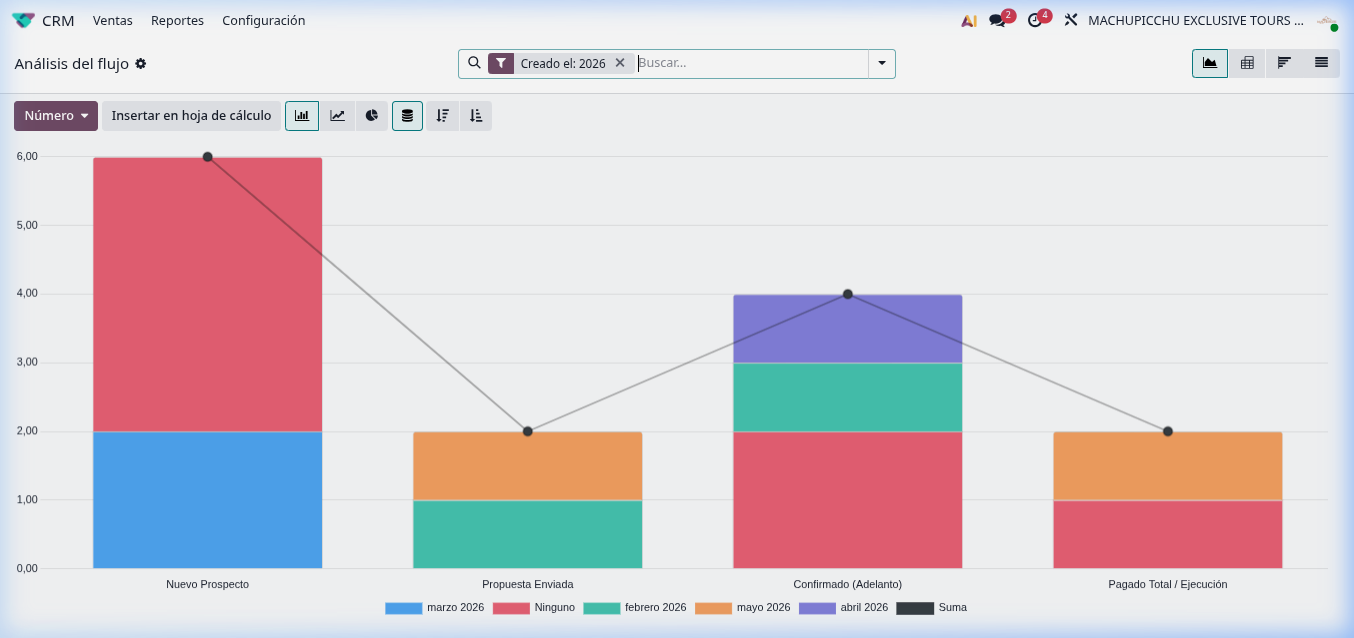
\includegraphics[width=\textwidth]{assets/odoo-crm-reportes-real.png}
    \caption{Reporte de análisis del flujo CRM por etapas en Odoo 19. Evidencia la distribución de oportunidades y la progresión del pipeline comercial (captura real del sistema, julio 2026).}
\end{figure}
\end{indentedsubsection}
